% tirlnx01 - Materiaal om het keuzevak Linux te geven 
% op de Hogeschool Rotterdam.
% Copyright (C) 2010 - 2011  Paul Sohier, Kevin van der Vlist
%
% This program is free software: you can redistribute it and/or modify
% it under the terms of the GNU General Public License as published by
% the Free Software Foundation, either version 3 of the License, or
% (at your option) any later version.
%
% This program is distributed in the hope that it will be useful,
% but WITHOUT ANY WARRANTY; without even the implied warranty of
% MERCHANTABILITY or FITNESS FOR A PARTICULAR PURPOSE.  See the
% GNU General Public License for more details.
%
% You should have received a copy of the GNU General Public License
% along with this program.  If not, see <http://www.gnu.org/licenses/>.
%
% Kevin van der Vlist - kevin@kevinvandervlist.nl
% Paul Sohier - paul@paulsohier.nl

\chapter{Installatie}\label{h.inst}
In dit complete dictaat is er gekozen voor de \emph{Slackware} distributie. Dit is gedaan omdat het een van de oudste, nog ``levende'' distributies binnen de \emph{Linux} wereld is, maar ook omdat je in \emph{Slackware} ontzettend veel zelf moet doen.

In dit hoofdstuk zal de lezer geholpen worden met het installeren van \emph{Slackware}, om precies te zijn met versie 13.37. De installatie kan plaatsvinden op een fysieke computer, maar ook het gebruik van \emph{VirtualBox} is erg handig. Zie voor het gebruik van \emph{Virtualbox} bijlage \ref{app.virtualbox}. 

Wanneer er een nieuwe versie van \emph{Slackware} uit is als de gebruikte versie in dit document is het altijd aan te raden deze nieuwe versie te gebruiken.

\section{Voordat we beginnen}
Voordat we beginnen met de installatie zijn we van het volgende uitgegaan bij het schrijven van dit dictaat;
\begin{itemize}
  \item We gaan er vanuit dat er geen data aanwezig is op de huidige harde schijf.
  \item We gaan er vanuit dat je gebruikt maakt van virtualbox, met een harde schijf van 25GiB. Maak je gebruik van een andere schijfgrote, zullen de commando's welke we gebruiken niet kloppen met wat jij moet uitvoeren.
  \item Als we een scherm niet bespreken of uitleggen, kan je gewoon de standaard waarde uit dat scherm aanhouden.
\end{itemize}

\section{Installatie starten} 
Stop de \emph{cd} van \emph{Slackware} in de \emph{cd-rom} speler en start op van \emph{cd-rom}. Via \emph{VirtualBox} zal de \emph{iso} eerste gemount moeten worden voordat de \emph{VM} wordt gestart. Er zal nu het een scherm komen zoals uit figuur \ref{fig:home}.

\begin{figure}[H]
  \begin{center}
    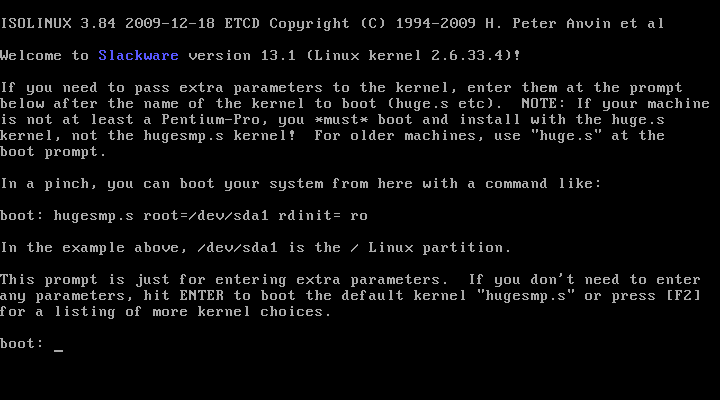
\includegraphics[scale=0.5]{images/09_home}
  \end{center}
  \caption{Voor het booten}
  \label{fig:home}
\end{figure}

Hier hoeft niets opgegeven te worden, er kan direct op enter gedrukt worden. Zodra er een  vraag wordt gesteld over de toetsenbord layout kan dit aangeven worden. Waarschijnlijk is het toetsenbord wat gebruikt wordt gewoon \emph{US-INTL}\footnote{Wanneer dit fout ingevult wordt kan dit later alsnog aangepast worden.} en kan er direct op enter gedrukt worden. Hierna dient er te worden ingelogd als ``root''. Type nu \texttt{setup}\index{setup}.

Zodra je setup hebt gekozen krijg wordt de fout uit figuur \ref{fig:fout} gegeven. Deze fout komt doordat er nog geen partities gemaakt zijn.
\begin{figure}[H]
  \begin{center}
    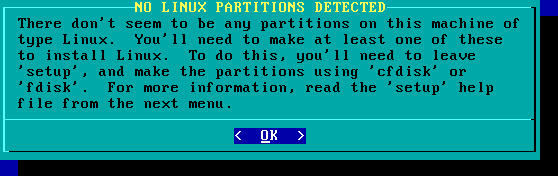
\includegraphics[scale=0.5]{images/08_installer_fout}
  \end{center}
  \caption{Fout bij het begin}
  \label{fig:fout}
\end{figure}

\section{fdisk}
Voordat we dus verder gaan moeten we eerst partities maken. Kies gewoon voor ``Ok'' en sluit de \emph{setup} af. Hierna kunnen we de partities als volgt aanmaken:
\begin{lstlisting}
fdisk /dev/sda
\end{lstlisting}
Waarbij \emph{/dev/sda} de harde schijf is welke gebruikt moet worden voor de \emph{Slackware} installatie. Voer de volgende commando's uit\footnote{Zie bijlage \ref{app.fdisk} voor meer informatie over \texttt{fdisk}\index{fdisk} en wat de onderstaande commando's/parameters betekenen.}:
\begin{lstlisting}
n
p
1
<default>
+10G
n
p
2
<default>
+14G
n
p
3
<default>
<default>
t
3
82
a
1
\end{lstlisting}
Controleer voordat de tabel wordt weggeschreven of dit klopt. Dit kan met de optie \emph{p}. Het zal overeen moeten komen met het onderstaande voorbeeld\footnote{Uiteraard er van uitgaande dat de harde schijf van dezelfde grote is. Controleer met de verhoudingen met de door jou gebruikte harde schijf.}:
\begin{lstlisting}
Command (m for help): p

Disk /dev/sda: 26.8 GB, 26843545600 bytes
255 heads, 63 sectors/track, 3263 cylinders, total 52428800 sectors
Units = sectors of 1 * 512 = 512 bytes
Sector size (logical/physical): 512 bytes / 512 bytes
I/O size (minimum/optimal): 512 bytes / 512 bytes
Disk identifier: 0x028f6a13

   Device Boot      Start         End      Blocks   Id  System
/dev/sda1   *        0       20973567    10485760   83  Linux
/dev/sda2        20973568    50333695    14680064   83  Linux
/dev/sda3        50333696    52428799     1047552   82  Linux swap
\end{lstlisting}
Wanneer het klopt kan de tabel met \emph{w} worden weggeschreven naar de schijf. De partitietabel is dan opgeslagen. \emph{Slackware} weet nu welke ruimte hij kan gebruiken. De installatie kan nu opnieuw gestart worden door het commando \texttt{setup} uit te voeren. 

\emph{Tip: Door de toets combinatie ``ctrl + page\_up'' en ``ctrl + page\_down'' kan door de terminal historie buffer gelopen worden}\index{historie}

\section{De installatie}
Nu begint de echte installatie van \emph{Slackware}. Het menu uit figuur \ref{fig:setup2} komt nu in beeld.
\begin{figure}[H]
  \begin{center}
    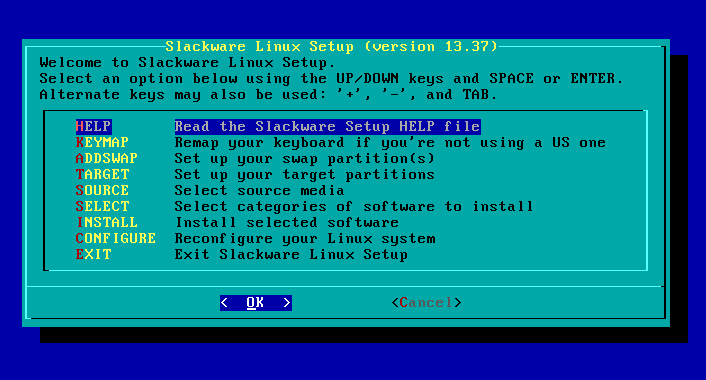
\includegraphics[scale=0.5]{images/01_installer}
  \end{center}
  \caption{Hoofdmenu van de installatie}
  \label{fig:setup2}
\end{figure}
De help functie hebben we niet nodig, omdat er al bekend is wat er gedaan moet worden. Het keyboard is ook al geconfigureerd, dus er kan gelijk gekozen worden voor de optie \emph{addswap}. Wanneer het bij \texttt{fdisk}\index{fdisk} goed is geconfigureerd zal hier \emph{/dev/sda3} weergeven worden. Kies hiervoor en druk op Ok. 

Er volgt nu een optie om op \emph{bad blocks} te controleren. In een \emph{VM} is dit niet nodig, bij fysieke hardware is het aan te raden om problemen te voorkomen. Hierna zal de \emph{swap} geactiveerd worden.

\subsection{Linux partities}
Er volgt nu een nieuw scherm, zoals te zien in figuur \ref{fig:partitie}\footnote{De waardes kunnen anders zijn, afhankelijk van de eerder gekozen waardes.}. \emph{Slackware} wil graag weten op welke partitie de \emph{root (/)} ge\"{i}nstalleerd kan worden. Kies hier voor \emph{/dev/sda1}, de kleinste van de twee. 

\begin{figure}[H]
  \begin{center}
    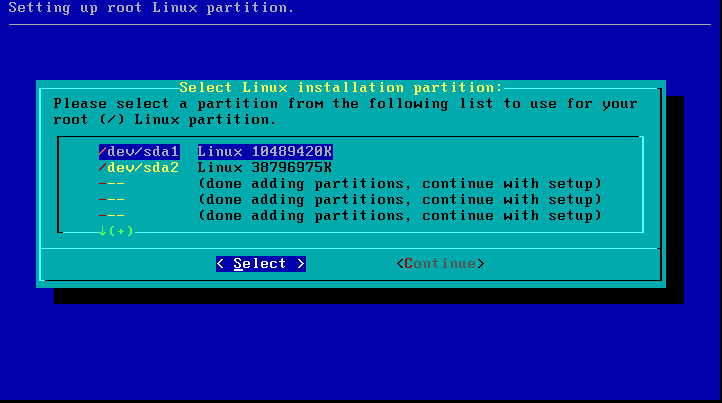
\includegraphics[scale=0.5]{images/02_partition}
  \end{center}
  \caption{Partities.}
  \label{fig:partitie}
\end{figure}

Bij de volgende stap moet het filesystem gekozen worden. Kies voor ``Format'' en in het volgende scherm het type, bijvoorbeeld \emph{EXT4}\index{EXT4}\footnote{Het gaat te ver om in dit document uitgebreid uit te leggen welke type file systems er zijn. \emph{EXT4} werkt in principe correct voor wat wij doen.}. Er kan nu weer een ``mount point'' worden gekozen. Kies hier voor \emph{/home}. Hierna zal er een overzicht te zien zijn, zoals figuur \ref{fig:fstab}.

\begin{figure}[H]
  \begin{center}
    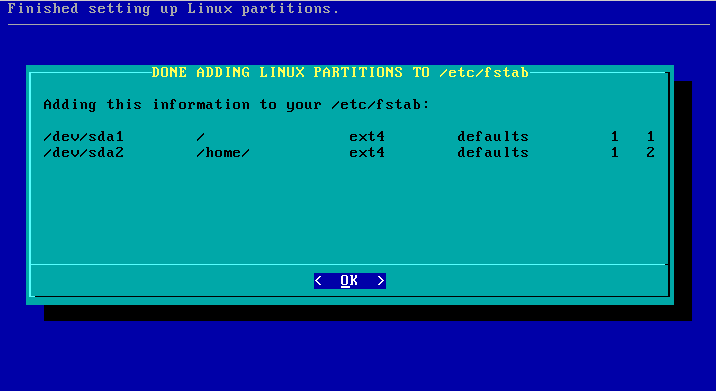
\includegraphics[scale=0.5]{images/03_fstab}
  \end{center}
  \caption{De gemaakte schijfindeling}
  \label{fig:fstab}
\end{figure}

\section{Packages}
De harde schijven zijn nu klaar voor gebruik en er kan begonnen met de installatie van het systeem. Zodra er op ``Ok'' wordt gedrukt zal er gevraagd worden om een locatie van de \emph{packages}. Kies hier voor \emph{FTP/HTTP}\footnote{CD is ook een mogelijkheid, alleen vereist het meer cd's}. Zie ook figuur \ref{fig:source}. 

\begin{figure}[H]
  \begin{center}
    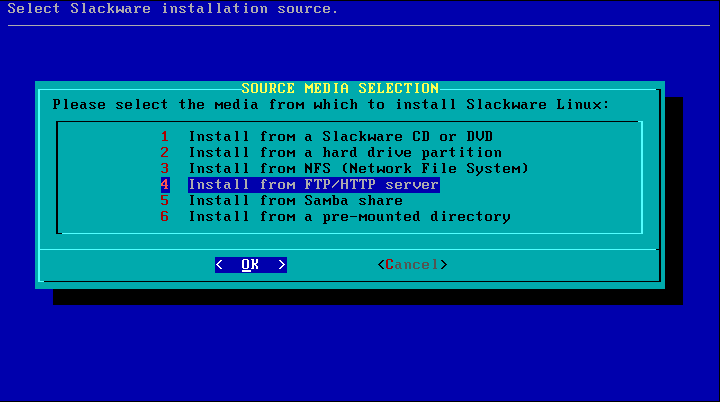
\includegraphics[scale=0.5]{images/04_source_media}
  \end{center}
  \caption{Source media keuze}
  \label{fig:source}
\end{figure}

Er zal nu worden gevraagd naar de netwerk configuratie. Dit is natuurlijk afhankelijk van de situatie. Bij het gebruik van \emph{VirtualBox} zal \emph{DHCP} voldoende zijn. Mocht je geen gebruik maken van \emph{Virtualbox} moet je de gegevens invullen welke voor het lokale netwerk gelden.

Er kan nu een \emph{mirror}\index{mirror} worden gekozen. Dit is een plek waar een kopie van alle \emph{Slackware} packages te vinden is. Een voorbeeld kan zijn \url{ftp://ftp.fu-berlin.de/}\footnote{Op de afbeelding is het IP van deze host te zien.}, zie ook \ref{fig:mirror}. Uiteraard kan ook een andere mirror gekozen worden. Zie hiervoor de \emph{Slackware} site.

\begin{figure}[H]
  \begin{center}
    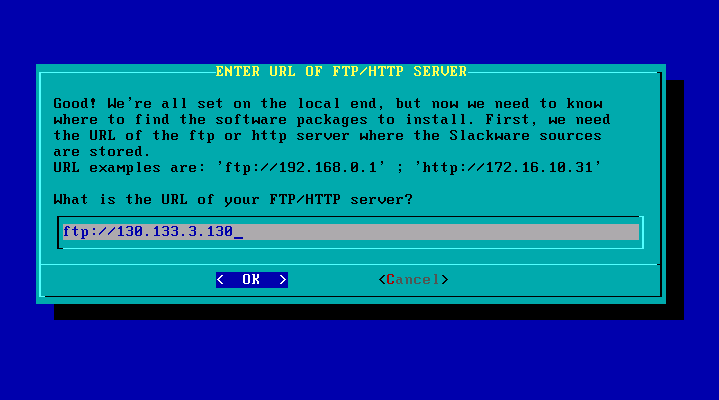
\includegraphics[scale=0.5]{images/05_mirror_location}
  \end{center}
  \caption{Mirror locatie}
  \label{fig:mirror}
\end{figure}

Nu zal er ook nog gekozen moeten worden voor een map op de \emph{mirror server}. Op het moment van schrijven is \emph{unix/linux/mirrors/slackware/slackware/} de goede directory. Dit kan bij het gebruik van een andere mirror een andere map zijn, dit is mirror afhankelijk. Zie hierbij ook figuur \ref{fig:mirror2}.

\begin{figure}[H]
  \begin{center}
    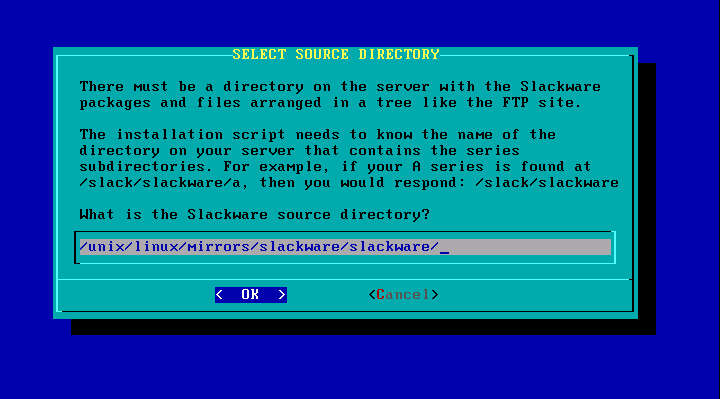
\includegraphics[scale=0.5]{images/06_mirror_location_2}
  \end{center}
  \caption{Mirror locatie}
  \label{fig:mirror2}
\end{figure}
\emph{Slackware} gaat nu controleren of de mirror gegevens kloppen en je krijgt, als de gegevens kloppen, de vraag of je het nogmaals wilt proberen of niet. Je kiest hier uiteraard voor niet. 

In dit scherm kan er gespecificeerd worden welke packages ge\"{i}nstalleerd moeten worden. De volgende packages zijn niet nodig, wij willen namelijk geen \emph{GUI} gebruiken. Deselecteer dus de volgende opties: 
\begin{itemize}
  \item[1.] Linux kernel source\footnote{Deze optie is alleen nodig als er kernels compiled worden op de machine}
  \item[2.] KDE
  \item[3.] TEX
  \item[4.] X
  \item[5.] XAP
  \item[6.] Games
\end{itemize}
Kies nu weer ``Ok'', zoals te zien op figuur \ref{fig:packages}. 

\begin{figure}[H]
  \begin{center}
    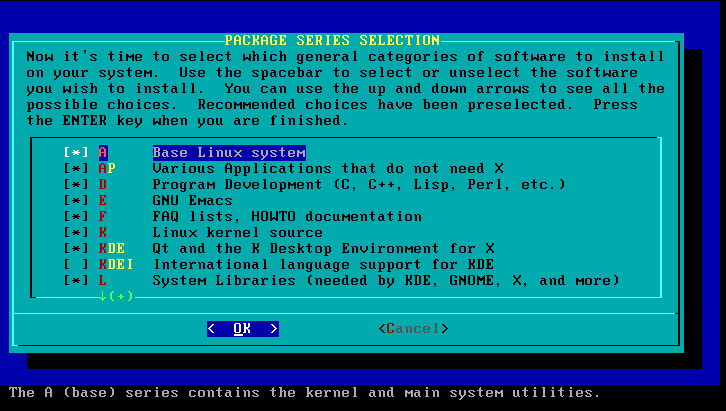
\includegraphics[scale=0.5]{images/07_package_select}
  \end{center}
  \caption{Packages}
  \label{fig:packages}
\end{figure}

Hierna krijg je het scherm zoals in figuur \ref{fig:install_full}. Het is aan te raden hier om ``full'' te kiezen, dit is de snelste optie en hoef je het minste te doen. Wanneer er een package vereist is om te installeren zal deze nu eerst automatisch van de gekozen \emph{mirror} afgehaald worden. Iedere package zal ook een korte beschrijving hebben welke op het scherm staat tijdens de installatie. Zodra \emph{Slackware} klaar is met alle packages op te halen en installeren gaat hij vanzelf verder met figuur \ref{fig:install_usb}. Op deze vraag kies je ``skip''.
\begin{figure}[H]
  \begin{center}
    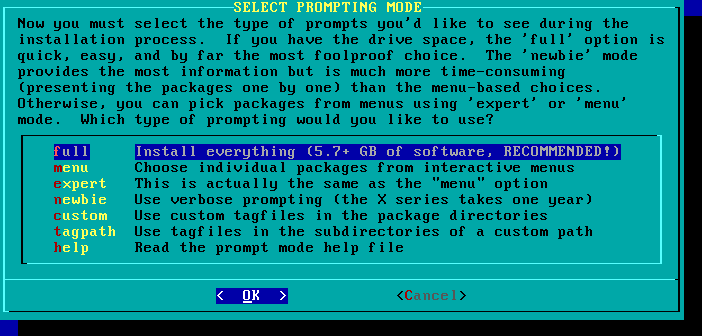
\includegraphics[scale=0.5]{images/install_full}
  \end{center}
  \caption{Installatie optie}
  \label{fig:install_full}
\end{figure}

\begin{figure}[H]
  \begin{center}
    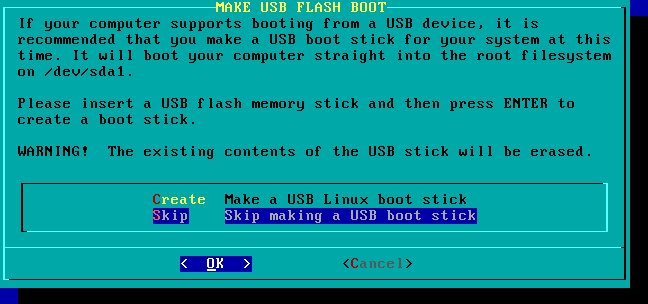
\includegraphics[scale=0.5]{images/install_usb}
  \end{center}
  \caption{USB opstart disk}
  \label{fig:install_usb}
\end{figure}


\section{LILO}
\begin{figure}[H]
  \begin{center}
    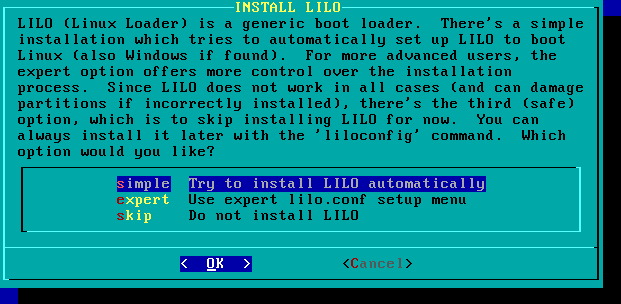
\includegraphics[scale=0.5]{images/install_lilo1}
  \end{center}
  \caption{LILO installatie}
  \label{fig:install_lilo1}
\end{figure}
\emph{LILO}\index{LILO} is de standaard bootmanager van \emph{Slackware}, \emph{LILO} is echter niet heel uitgebreid en je kan er niet veel mee. Hierom hebben wij ervoor gekozen om \emph{GRUB}\index{GRUB} te gaan gebruiken als bootmanager en gaan we deze later dan ook installeren. Maar voordat we dit kunnen, moeten we eerst een werkend systeem hebben en moet je dus \emph{LILO} installeren. 

In het scherm van \ref{fig:install_lilo1} moet je ``simple'' kiezen. Hierna krijg je het scherm uit figuur \ref{fig:install_lilo2}. Je kan hier de standaard instelling behouden.

\begin{figure}[H]
  \begin{center}
    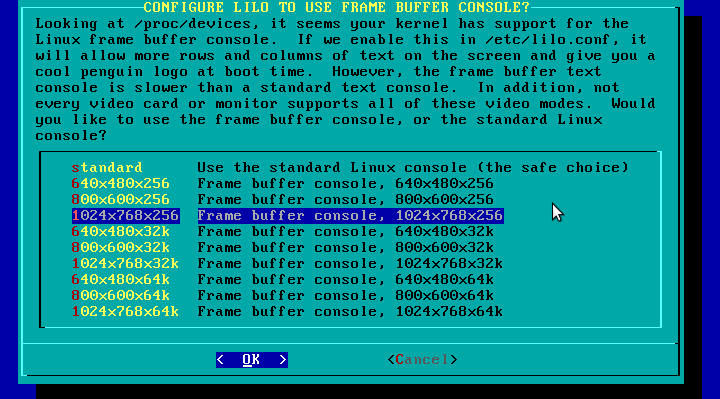
\includegraphics[scale=0.5]{images/install_lilo2}
  \end{center}
  \caption{LILO framebuffer}
  \label{fig:install_lilo2}
\end{figure}

\begin{figure}[H]
  \begin{center}
    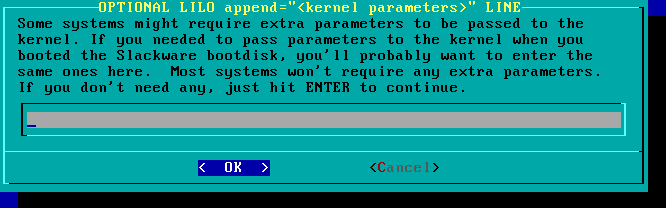
\includegraphics[scale=0.5]{images/install_lilo3}
  \end{center}
  \caption{LILO kernel options}
  \label{fig:install_lilo3}
\end{figure}
\begin{figure}[H]
  \begin{center}
    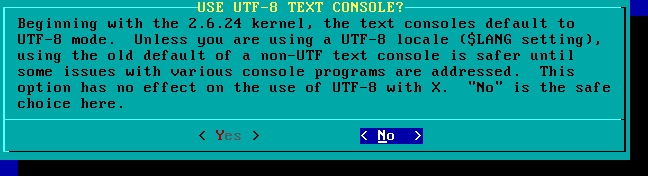
\includegraphics[scale=0.5]{images/install_lilo4}
  \end{center}
  \caption{LILO UTF8}
  \label{fig:install_lilo4}
\end{figure}
In sommige gevallen is het nodig om de kernel een aantal extra opties mee te geven om op te starten. Dit kan je in de installatie opgeven in \ref{fig:install_lilo3}. In principe hoef je hier niets op te geven en werkt het direct. Voor de echte instellingen krijgen we eerst nog een vraag over UTF8 zoals uit figuur \ref{fig:install_lilo4}. Je kan hier gewoon het standaard antwoord kiezen.

\begin{figure}[H]
  \begin{center}
    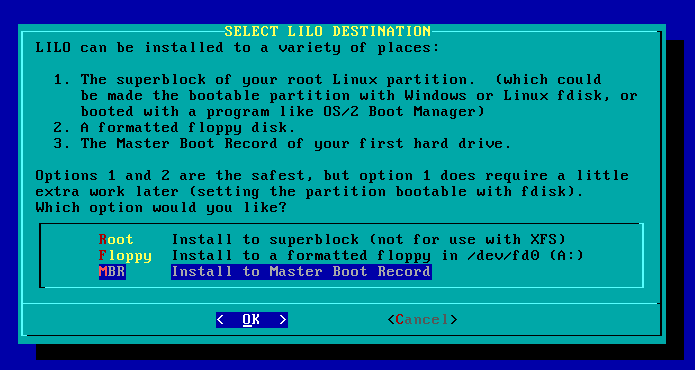
\includegraphics[scale=0.5]{images/install_lilo5}
  \end{center}
  \caption{LILO locatie}
  \label{fig:install_lilo5}
\end{figure}
In het scherm van figuur \ref{fig:install_lilo5} wordt gevraagd waar \emph{LILO} geinstalleerd moet worden. Je kan hier kiezen voor \emph{mbr}, de standaard keuze. In principe kan je ook kiezen voor \emph{root}, mits je de partitie als \emph{bootable} hebt ingesteld. Als je de instructies correct gevolgd heb was hij al bootable.

\section{Laatste configuratie}
Kies als muis voor een generieke \emph{PS2} muis. Dit zal de minste kans op problemen geven. 
Er zal ook nu weer om de netwerk configuratie gevraagd worden. Vul deze weer op de gewenste manier in. Vul als hostname een zelf gekozen naam in.

Op de vraag over welke \emph{services} geactiveerd moeten zijn kan er gewoon met ``Ok'' de default waardes worden bevestigd. Als tijdzone kan er natuurlijk gewoon ``Europe/Amsterdam'' worden gekozen, tenzij er een andere waarde gewenst is. 

Om het systeem veilig te kunnen gebruiken is het nodig om een \emph{root wachtwoord} op te geven. Dit wachtwoord is nodig om als hoofdgebruiker op het systeem in te kunnen loggen en zal dus een veilig en sterk wachtwoord moeten zijn. Onthoud en bescherm dit goed! 

Na een herstart (\texttt{reboot}\index{fdisk}) kan er ingelogd worden met ``root'' en het gekozen wachtwoord. 

\section{GRUB installatie}
De standaard bootloader van \emph{Slackware} is \emph{LILO}. Omdat \emph{GRUB} gemakkelijker en uitgebreider is, gaan we in dit dictaat gebruik maken van \emph{GRUB}.

\subsection{Downloaden en installeren GRUB}
In het geval van \emph{GRUB} bestaat er een standaard package om te installeren, maar staat deze enkel in ``extra''. Dit kunnen we vinden in de \emph{PACKAGES.TXT}\footnote{\url{ftp://ftp.fu-berlin.de/unix/linux/mirrors/slackware/slackware-13.37/extra/PACKAGES.TXT}}. Download de \emph{package}, en installeer deze: 
\begin{lstlisting}
root@slackbak:~# cd /tmp/
root@slackbak:/tmp# wget "ftp://ftp.fu-berlin.de/unix/linux/mirrors/slackware/slackware/extra/grub/grub-0.97-i486-9.txz"
root@slackbak:/tmp# installpkg grub-0.97-i486-9.txz 
\end{lstlisting}

\subsection{grubconfig}
\emph{GRUB} is nu ge\"{i}nstalleerd, maar nog niet geconfigureerd. Voordat \emph{GRUB} gebruik kan worden zal dat eerst gedaan moeten worden. Dit is echter erg eenvoudig:
\begin{lstlisting}
grubconfig
\end{lstlisting}
Hierna krijg je de zelfde soorten vragen als bij \emph{LILO}, je kan hier ook dezelfde antwoorden invullen.

De installatie is nu helemaal afgerond. Wanneer er gebruik wordt gemaakt van \emph{VirtualBox} is het aan te raden een kopie te maken van de harde schijf. Wanneer er dan iets fout gaat, kan simpelweg de kopie van de schijf worden teruggezet. Dit scheelt een herinstallatie van \emph{Slackware}. 
